% pour genree un pdf: faire
% pdflatex exemple.tex
\documentclass{article}

%% Paquets LateX utiles

\usepackage[utf8]{inputenc} 		% encodage des caracteres utilise (pour les caracteres accentues) -- non utilise ici.
%\usepackage[latin1]{inputenc} 		% autre encodage
\usepackage[french]{babel}		% pour une mise en forme "francaise"
\usepackage[T1]{fontenc} 
\usepackage{amsmath,amssymb,amsthm}	% pour les maths
\usepackage{graphicx}			% pour inclure des graphiques

\usepackage[hidelinks]{hyperref}
\usepackage{color}			% pour ajouter des couleurs dans vos textes
\usepackage{geometry}
\geometry{hmargin=2.5cm,vmargin=3cm}
\renewcommand{\contentsname}{\centering Contents}


\begin{document}
\begin{titlepage}
    \begin{flushleft}
    
\includegraphics[width=11em]{logo.png}\\[1.5cm]
    \end{flushleft}
    \begin{center}
        \textsc{{\LARGE \color{blue} Master Données, Apprentissage et Connaissances-DAC}}\\[5cm]
        \textsc{\Huge{CARNET DE BORD}}\\[1cm]
        \textbf{\Large{Sujet:}}
        \textsc{\large{Problème de clustering pour les infrastructures sans fil.}}\\[6cm]
        \begin{minipage}{1\textwidth}
            \begin{flushleft} \large
            \textsc{\LARGE{Realisé par :}}\\[0.5cm]
            \textsc{Liticia TOUZARI}\\
            \textsc{Hanane DJEDDAL}\\[1.5 cm]
            \end{flushleft}
        \end{minipage}
        \vfill
    \end{center}
  \end{titlepage}
  

\tableofcontents%  Table des matieres


\newpage

\vspace*{\stretch{0.5}}
  \begin{center}
\section*{\LARGE{Introduction}}
  \end{center}
\Large{\paragraph{}
        Aujourd'hui, le trafic de données sur les réseaux mobiles connaît une croissance explosive à mesure que les smartphones et tablettes compatibles avec Internet deviennent de plus en plus populaires.\\
Afin de répondre à la demande croissante de trafic de données, les opérateurs de réseaux mobiles doivent augmenter leur capacité de traitement de données, comme le déploiement de plus de stations de base et l'ajout d'unités de traitement de données supplémentaires aux stations de base. \\
Cependant, les dépenses en capital liées au déploiement de ces infrastructures de réseau deviennent de plus en plus élevées. Par conséquent, l'optimisation des dépenses d'investissement et des dépenses d'exploitation tout en maintenant une qualité de service est devenue une nécessité pour les opérateurs de réseaux mobiles.
\paragraph{}
Ce projet vise à mettre en œuvre des techniques de clustering afin de regrouper les ressources et infrastructures radio dans le but d'améliorer l'efficacité des services. 
Chaque ville est desservie par plusieurs nœuds sans fil qui sont géographiquement séparés; chacun d'eux est responsable d'une charge différente des appels vocaux, de la consommation multimedia et des messages provenant de différentes zones de la ville dans la journée. 
À ce jour, les différents nœuds d'accès du réseau ne coopèrent pas, et chaque nœud est plutôt responsable de sa propre zone géographique. Les architectures futures des réseaux proposent de regrouper plusieurs stations sans fil et les traiter comme un ensemble avec un contrôleur commun, afin que les stations surchargées puissent être soutenues par des stations sous-chargées. 
\paragraph{}
Dans le cadre de ce projet, on proposera des méthodes de clustering efficaces, adaptées aux spécificités de l'environnement sans fil et des métriques des services de télécommunications. On utilisera des données fournies par l’opérateur Orange.
}
\vspace*{\stretch{1}}
\newpage

\section{Travail attendu}
\paragraph{}
 Le projet est divisé en une séquence trois grandes taches principales à réaliser : \\
\begin{itemize}
    \item Étude bibliographique et état de l'art. 
    \item Proposition de différents schémas de clustering pour améliorer la qualité de service et l'équité des ressources. En incluent des aspects de performance télécom aux méthodes préexistantes.
    \item Application des méthodes proposées de clustering aux données réels de telecom afin d'évaluer leur efficacité dans les exemples de réseaux réels.
\end{itemize}

\section{Mots clés retenus}
\begin{flushleft}
Le schéma ci-dessous représente les mots clés utilisés dans ce projet sous forme d'une carte heuristique :\\
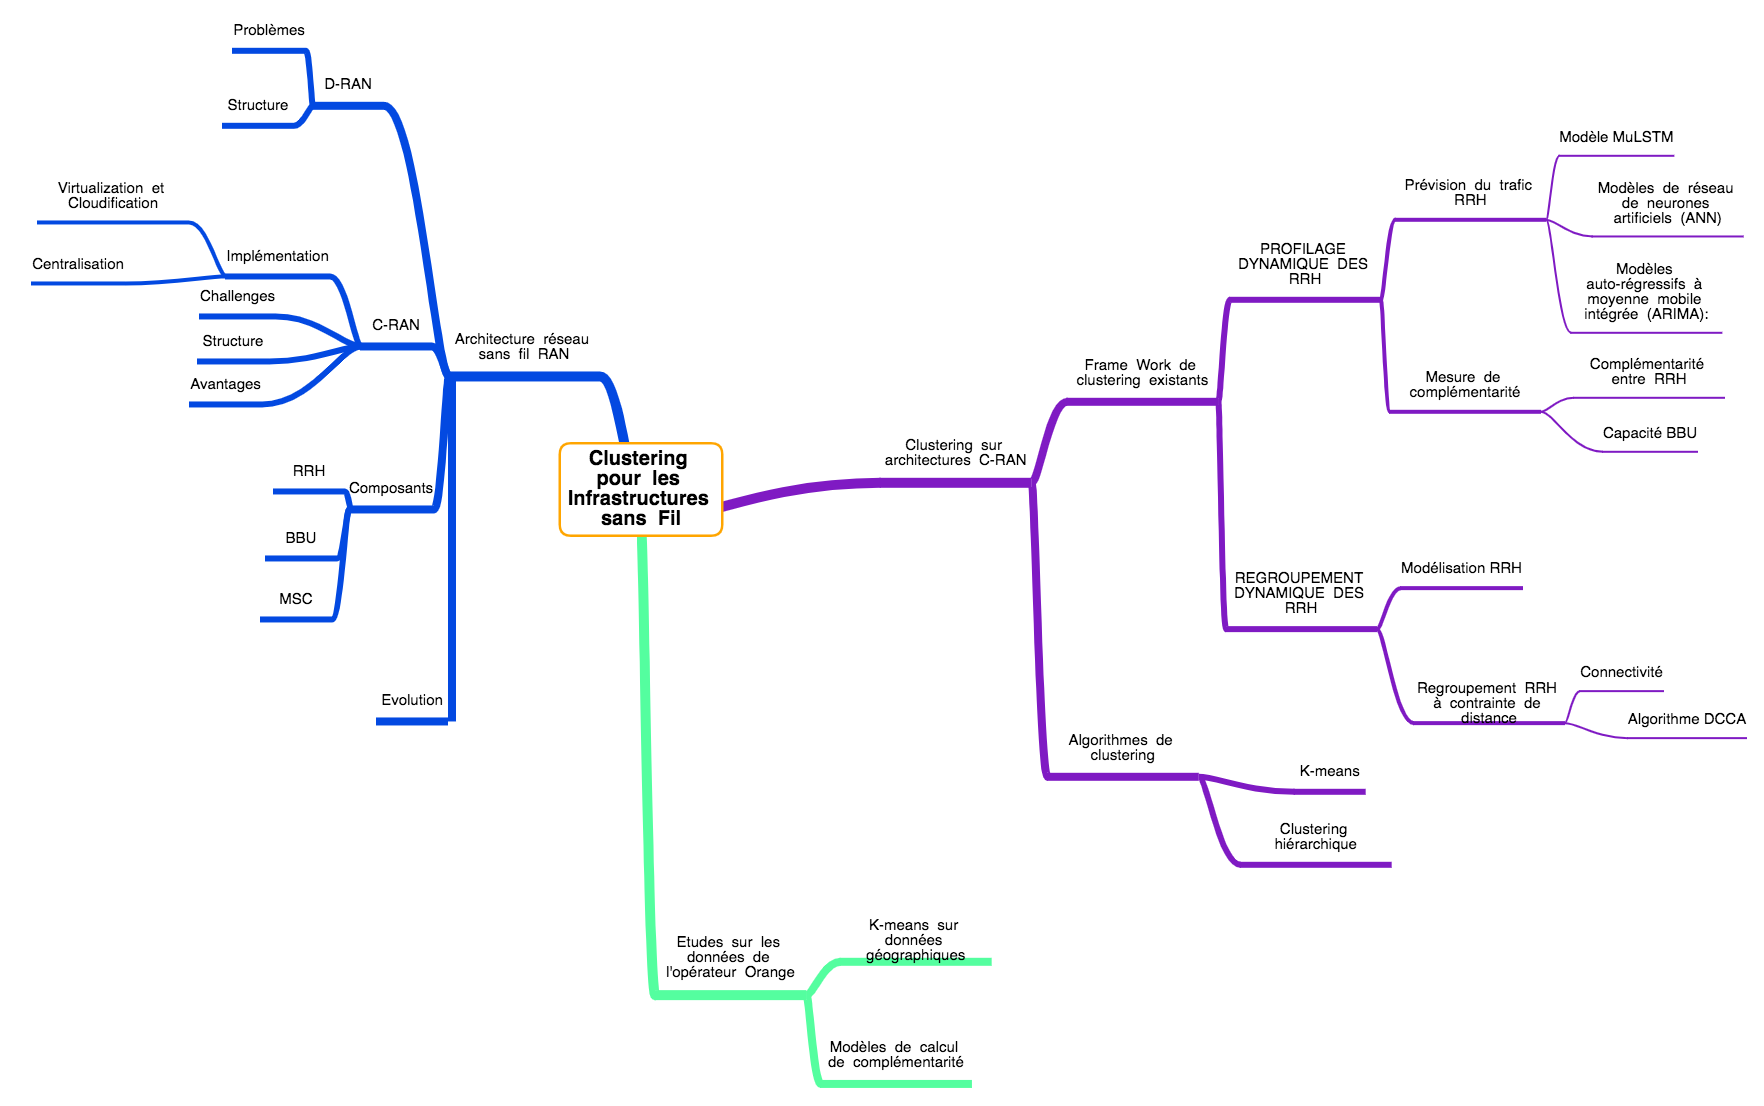
\includegraphics[width=38em]{schema.png}\\[1.5cm]
\end{flushleft}
\section{Descriptif de la recherche documentaire}
\paragraph{}
La recherche documentaire était principalement dévisée en deux grandes parties : 
l’étude de l’architecture C-RAN et l’étude des algorithmes de clustering.\\
Les articles fournis par l’encadreur étaient le point de départ et la référence 
de base qui a guidé la recherche. \\
Dans un premier temps, le but était d’avoir une compréhension général du domain : Réseau. 
Pour cela, on a utilisé des pages web telles que Wikipedia, Whatis.techtarget, Comment ça marche 
etc, ainsi que des videos YouTube pour avoir des définitions des termes, des exemples et des 
explications simplifiées. Par la suite, on a adopté une recherche par mots clés sur google 
scholar, ieeexplore.ieee.org et le moteur de recherche SUper, pour étudier les architectures 
RAN existants et la migration vers le cloud-RAN. On a pu obtenir des ressources en ligne telles 
que des thèses de recherches, des revues et des articles de journal.\\
Pour la deuxième partie, l’étude sur les algorithmes de clustering général était basée sur le chapitre 10.3 du livre “An introduction to Statistical Learning” et le cours “NDA: Clustering” fournis par l’encardreur; ainsi que les cours du UE: ‘sciences des données’ de licence 3 informatique. Ensuite, en suivant la même approche que la premère partie, on a etudié les algorithmes de clustering proposés pour les architectures C-RAN.
\section{Bibliographie produite dans le cadre du projet}
\paragraph{}Bibliographie générée depuis Zotero avec norme ACM : \\
\begin{enumerate}
\item[{[1]}] Brown, G. 2017. Cloud RAN & the Next-Generation Mobile Network Architecture. (2017), 9.
\item[{[2]}] Checko, A. et al. 2015. Cloud RAN for Mobile Networks—A Technology Overview. IEEE Communications Surveys & Tutorials. 17, 1 (2015), 405–426. DOI:https://doi.org/10.1109/COMST.2014.2355255.
\item[{[3]}] Chen, L. et al. 2018. Deep mobile traffic forecast and complementary base station clustering for C-RAN optimization. Journal of Network and Computer Applications. 121, (Nov. 2018), 59–69. DOI:https://doi.org/10.1016/j.jnca.2018.07.015.
\item[{[4]}] I, C.-L. et al. 2014. Recent Progress on C-RAN Centralization and Cloudification. IEEE Access. 2, (2014), 1030–1039. DOI:https://doi.org/10.1109/ACCESS.2014.2351411.
\item[{[5]}] James, G. et al. 2013. An Introduction to Statistical Learning. Springer New York.
\item[{[6]}] Jaziri, A. et al. 2017. Tracking Traffic Peaks in Mobile Networks Using Statistics of Performance Metrics. International Journal of Wireless Information Networks. 24, 4 (Dec. 2017), 389–403. DOI:https://doi.org/10.1007/s10776-017-0335-6.
\item[{[7]}] Khan, M. et al. 2017. QoS-Aware Dynamic RRH Allocation in a Self-Optimized Cloud Radio Access Network With RRH Proximity Constraint. IEEE Transactions on Network and Service Management. 14, 3 (Sep. 2017), 730–744. DOI:https://doi.org/10.1109/TNSM.2017.2719399.
\item[{[8]}] Lee, D. et al. 2012. Coordinated multipoint transmission and reception in LTE-advanced: deployment scenarios and operational challenges. IEEE Communications Magazine. 50, 2 (Feb. 2012), 148–155. DOI:https://doi.org/10.1109/MCOM.2012.6146494.
\item[{[9]}] Novaes, C. et al. 2020. Virtualized C-RAN Orchestration with Docker, Kubernetes and OpenAirInterface. arXiv:2001.08992 [eess]. (Jan. 2020).
\item[{[10]}] Han, B. et al. 2019. Research on Resource Migration Based on Novel RRH-BBU Mapping in Cloud Radio Access Network for HSR Scenarios. IEEE Access. 7, (2019), 108542–108550. DOI:https://doi.org/10.1109/ACCESS.2019.2933567.
\item[{[11]}] Wu, J. et al. 2015. Cloud radio access network (C-RAN): a primer. IEEE Network. 29, 1 (Jan. 2015), 35–41. DOI:https://doi.org/10.1109/MNET.2015.7018201.
\item[{[12]}] Wu, Z. and Wu, Z. 2020. An Enhanced Regularized k-Means Type Clustering Algorithm With Adaptive Weights. IEEE Access. 8, (2020), 31171–31179. DOI:https://doi.org/10.1109/ACCESS.2020.2972333.
\end{enumerate}
\section{Évaluation des sources}
\begin{itemize}
  \item [{[4]}] Recent Progress on C-RAN Centralization and Cloudification :
  \paragraph{}

  Cet article, fourni par l’encadreur, date de 2014, 4ans après l’introduction 
  de l’architecture C-RAN par China Mobile Research Institute (CMRI). Il donne les 
  derniers progrès dans cette technologie ainsi que les choix d’implementations et 
  les améliorations possibles. Parmi les auteurs de cet article : la chargée de la 
  recherche et dévelopement des réseaux sans fils avancées de CRMI , ainsi que 2 chefs 
  de projets à CMRI et le directeur de The Green Communications Research Center de CMRI. 
  Le projet étant basé sur le clustering dans les architectures C-RAN, une bonne compréhension 
  de la technologie était un point crutial, et donc cet article, le travail direct d’une équipe 
  de l’institut où la technologie a émergé, était une source importante pour guider la recherche.
  
  \item [{[8]}] Coordinated multipoint transmission and reception in LTE-advanced: deployment scenarios and operational challenges
  \paragraph{}
  En un niveau plus détaillé dans la recherche, il était essentiel de comprendre la communications 
  entre RRHs et le fonctionnement des antennes afin de pouvoir critiquer les algorithmes proposés. Cet article 
  explique la technique de coopération Coordinated Multipoint transmission (CoMP) et prévoit l'utilité 
  de cette technique dans les technologies avancées. Publié dans IEEE communications magazine en 2012, 
  cet article est cité 730 fois sur google scholar, 407 fois sur web of science, 474 fois sur Scopus et 447 fois 
  sur Crossref avec un total d'utilisation, qui inclus le telechargement de PDF et HTML views, de 11108 depuis 
  2012, 54 fois étant en 2020 et 39 fois en 2019 ce qui atteste qu'il est encore d'actualité. L'artcile,
   qui engendre une étude expérimentale était le travail d'une équipe des chercheurs qui ont contribués dans le
   developement de la technologie LTE et qui viennent de différents groupes specilisés en telecommunication tels que 
   Orange, Samsung Electronics, LG Electronics, Huawei technologies etc. Ce qui implique une très bonne fiabilité.
  
   \item [{[12]}] An Enhanced Regularized k-Means Type Clustering Algorithm With Adaptive Weights:
   \paragraph{}
  Cet article, disponible sur IEEE digital Library et publié dans le journal IEEE Access en février 2020
  a un lien direct avec l'objectif du projet. Enfait, il propose un variante de l'algorithme K-means qui introduit
   la notion de poids, chose qui peut être utile dans le contexte de télécommunication. Selon les métriques de 
   pertinence, l'article n'était pas cité, ce qui est justifié par sa date de publication très récente. Les auteurs 
   sont des nouveaux diplomés de PH.D (2018 et 2019) dans le domaine d'electronique. Cependant, le contenu 
   de l'article est, consistant, offrant des démonstrations mathématiques ainsi qu'une évaluation 
   expérimentale. Ses références étaient aussi vérifiable (accessible en ligne et/ou sur google scholar).

   \vspace*{\stretch{0.5}}
   \begin{center}
 \section*{\LARGE{Conclusion}}
   \end{center}
 \Large{\paragraph{}
 Dans ce carnet de bord, on a exposé la méthode suivie et les moyens utlisés afin d'assurer une bonne 
 recherche documentaire. Après avoir dressé une carte heuristique pour bien encadrer le projet et déterminer
 les mots clés, on a utilisé des différents outils pour obtenir des sources d'information. Le choix 
 d'outil dépendait du type d'information desirée. A la fin, une évaluation des sources selon des 
 métriques définis, a permis de juger la fiabilité de l'information et par la suite garantir la fiabilité de notre travail. 
 }
 \vspace*{\stretch{1}}
\end{document}